\documentclass[a4paper,10pt,DIV=14]{article}
\usepackage{graphicx}
\usepackage[utf8]{inputenc} % korrekte Darstellung von Umlauten u. Sonderzeichen
\usepackage[ngerman]{babel} % Sprachpaket, ngerman = neue deutsche Rechtschreibung
\usepackage{amsmath} % Setzen mathematischer Formeln
\usepackage{amsfonts} %mathbb
\usepackage{titlesec}
\usepackage{float}
\usepackage{caption}
\usepackage{fancyvrb}
\usepackage{siunitx}
\usepackage{booktabs}
\usepackage{enumitem}

\usepackage{tabularx}
\newcolumntype{L}[1]{>{\raggedright\arraybackslash}p{#1}} % linksbündig mit Breitenangabe
\newcolumntype{C}[1]{>{\centering\arraybackslash}p{#1}} % zentriert mit Breitenangabe
\newcolumntype{R}[1]{>{\raggedleft\arraybackslash}p{#1}} % rechtsbündig mit Breitenangabe

\newcommand{\gqq}[1]{\glqq{}#1\grqq{}}
\newcommand{\gq}[1]{\glq{}#1\grq{}}
\newcommand{\dg}[1]{#1^\circ}

\renewcommand{\thesection}{Aufgabe \arabic{section}:}
\renewcommand{\thesubsection}{\alph{subsection})}

\titleformat{\subsection}
{\normalsize}{\thesubsection}{1em}{}


\captionsetup[figure]{labelformat=empty}


\begin{document}

\title{Graphische Datenverarbeitung WS17/18 \\ Theorieübung 2}
\author{
  Salmah Ahmad (2880011)
  \and
  Markus Höhn (1683303)
  \and
  Tobias Mertz (2274355)
  \and
  Steven Lamarr Reynolds (1620638)
  \and
  Sascha Zenglein (2487032)
}

\maketitle

\section{Transformation}

\subsection{Berechnen Sie die vollständigen 4x4 Transformationsmatrizen $M^A(\alpha)$ und $M^B(\alpha)$ für die Zahnräder A und B in Abhängigkeit von $\alpha$}

\begin{figure}[!htbp]
	\centering
	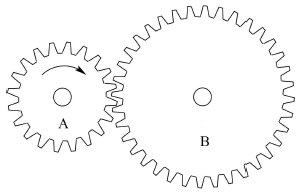
\includegraphics[]{gear}
\end{figure}

\begin{align*}
M^A(\alpha) & = \begin{pmatrix}
					1 & 0 & 0 & 5 \\
					0 & 1 & 0 & 7 \\
					0 & 0 & 1 & 5 \\
					0 & 0 & 0 & 1 \\
				\end{pmatrix} \cdot
				\begin{pmatrix}
					1 & 0             & 0              & 0 \\
					0 & \cos(-\alpha) & -\sin(-\alpha) & 0 \\
					0 & \sin(-\alpha) & \cos(-\alpha)  & 0 \\
					0 & 0             & 0              & 1 \\
				\end{pmatrix} \cdot
				\begin{pmatrix}
					1 & 0 & 0 & -5 \\
					0 & 1 & 0 & -7 \\
					0 & 0 & 1 & -5 \\
					0 & 0 & 0 & 1  \\
				\end{pmatrix} \\
			& = \begin{pmatrix}
					1 & 0 & 0 & 5 \\
					0 & 1 & 0 & 7 \\
					0 & 0 & 1 & 5 \\
					0 & 0 & 0 & 1 \\
				\end{pmatrix} \cdot
				\begin{pmatrix}
					1 & 0             & 0              & -5                               \\
					0 & \cos(-\alpha) & -\sin(-\alpha) & -7\cos(-\alpha) + 5\sin(-\alpha)  \\
					0 & \sin(-\alpha) & \cos(-\alpha)  & -7\sin(-\alpha) - 5\cos(-\alpha) \\
					0 & 0             & 0              & 1                                \\
				\end{pmatrix} \\
			& = \begin{pmatrix}
					1 & 0             & 0              & 0                                    \\
					0 & \cos(-\alpha) & -\sin(-\alpha) & -7\cos(-\alpha) + 5\sin(-\alpha) + 7  \\
					0 & \sin(-\alpha) & \cos(-\alpha)  & -7\sin(-\alpha) - 5\cos(-\alpha) + 5 \\
					0 & 0             & 0              & 1                                    \\
				\end{pmatrix}
\end{align*}

mit $Z_A = \frac{-\alpha}{360} \cdot 20$ und $\beta = \frac{Z_A}{50} \cdot 360$ gilt:
$$ \beta = \frac{- \alpha * 20 \cdot 360}{360 \cdot 50} = -0.4 \alpha$$

\begin{align*}
	M^B(\alpha) & = \begin{pmatrix}
						1 & 0 & 0 & 5 \\
						0 & 1 & 0 & 7 \\
						0 & 0 & 1 & 2 \\
						0 & 0 & 0 & 1 \\
					\end{pmatrix} \cdot
					\begin{pmatrix}
						1 & 0                & 0                 & 0 \\
						0 & \cos(-0.4\alpha) & -\sin(-0.4\alpha) & 0 \\
						0 & \sin(-0.4\alpha) & \cos(-0.4\alpha)  & 0 \\
						0 & 0                & 0                 & 1 \\
					\end{pmatrix} \cdot
					\begin{pmatrix}
						1 & 0 & 0 & -5 \\
						0 & 1 & 0 & -7 \\
						0 & 0 & 1 & -2 \\
						0 & 0 & 0 & 1  \\
					\end{pmatrix} \\
				& = \begin{pmatrix}
						1 & 0 & 0 & 5 \\
						0 & 1 & 0 & 7 \\
						0 & 0 & 1 & 2 \\
						0 & 0 & 0 & 1 \\
					\end{pmatrix} \cdot
					\begin{pmatrix}
						1 & 0                & 0                 & -5                                     \\
						0 & \cos(-0.4\alpha) & -\sin(-0.4\alpha) & -7\cos(-0.4\alpha) + 2\sin(-0.4\alpha) \\
						0 & \sin(-0.4\alpha) & \cos(-0.4\alpha)  & -7\sin(-0.4\alpha) - 2\cos(-0.4\alpha) \\
						0 & 0                & 0                 & 1                                      \\
					\end{pmatrix} \\
				& = \begin{pmatrix}
						1 & 0                & 0                 & 0                                          \\
						0 & \cos(-0.4\alpha) & -\sin(-0.4\alpha) & -7\cos(-0.4\alpha) + 2\sin(-0.4\alpha) + 7 \\
						0 & \sin(-0.4\alpha) & \cos(-0.4\alpha)  & -7\sin(-0.4\alpha) - 2\cos(-0.4\alpha) + 2 \\
						0 & 0                & 0                 & 1                                          \\
					\end{pmatrix}
\end{align*}

\section{Baryzentrische Koordinaten}

\subsection{Gegeben sei ein Tetraeder $T = [p_0, p_1, p_2, p_3]$ mit $p_0 = (0, 0, 0)^T$, $p_1 = (-2, 1, 0)^T$, $p_2 = (0, 5, 1)^T$ und $p_3 = (-1, 2, 4)^T$. \vspace{.5em} \\  Berechnen Sie die baryzentrischen Koordinaten $\lambda_i, i = 0, 1, 2, 3$ für den Punkt $p = (-1, 2, 2)^T$. Verwenden Sie dafür die Determinanten der Matrizen folgender Form:}
	$$M = \begin{pmatrix}
	\begin{bmatrix}0\\0\\0\end{bmatrix} & \begin{bmatrix}-2\\1\\0\end{bmatrix} & \begin{bmatrix}0\\5\\1\end{bmatrix} & \begin{bmatrix}-1\\2\\4\end{bmatrix} \\
	1   & 1   & 1   & 1   \\
	\end{pmatrix}$$


\begin{align*}
	\det M & = 0 \cdot	\begin{vmatrix}
							1 & 5 & 2 \\
							0 & 1 & 4 \\
							1 & 1 & 1 \\
						\end{vmatrix}
		 - (-2) \cdot	\begin{vmatrix}
						 	0 & 5 & 2 \\
						 	0 & 1 & 4 \\
						 	1 & 1 & 1 \\
						\end{vmatrix}
		 + 0 \cdot		\begin{vmatrix}
						 	0 & 1 & 2 \\
						 	0 & 0 & 4 \\
						 	1 & 1 & 1 \\
						\end{vmatrix}
		 - (-1) \cdot	\begin{vmatrix}
		 					0 & 1 & 5 \\
		 					0 & 0 & 1 \\
		 					1 & 1 & 1 \\
						\end{vmatrix} \\
	       & = 0 \cdot 15 + 2 \cdot 18 + 0 \cdot 4 + 1 \cdot 1 \\
	       & = 37
\end{align*}

\begin{alignat*}{3}
	L_0 = \begin{vmatrix}
				-1 & -2 &  0 & -1 \\
			 2 &  1 &  5 &  2 \\
			 2 &  0 &  1 &  4 \\
			 1 &  1 &  1 &  1 \\
			\end{vmatrix} = 4
	& \qquad \Rightarrow \qquad
	& \lambda_0 = \frac{L_0}{\det M} = \frac{4}{37} \\
	L_1 = \begin{vmatrix}
				0 & -1 &  0 & -1 \\
				0 &  2 &  5 &  2 \\
				0 &  2 &  1 &  4 \\
				1 &  1 &  1 &  1 \\
	 	  \end{vmatrix} = 10
	& \qquad \Rightarrow \qquad
	& \lambda_1 = \frac{L_1}{\det M} = \frac{10}{37} \\
	L_2 = \begin{vmatrix}
				0 & -2 & -1 & -1 \\
				0 &  1 &  2 &  2 \\
				0 &  0 &  2 &  4 \\
				1 &  1 &  1 &  1 \\
			\end{vmatrix} = 6
	& \qquad \Rightarrow \qquad
	& \lambda_2 = \frac{L_2}{\det M} = \frac{6}{37} \\
	L_3 = \begin{vmatrix}
				0 & -2 &  0 & -1 \\
				0 &  1 &  5 &  2 \\
				0 &  0 &  1 &  2 \\
				1 &  1 &  1 &  1 \\
			\end{vmatrix} = 17
	& \qquad \Rightarrow \qquad
	& \lambda_3 = \frac{L_3}{\det M} = \frac{17}{37} \\
\end{alignat*}

$$ p_{BAR} = \left( \frac{4}{37}, \frac{10}{37}, \frac{6}{37}, \frac{17}{37} \right)  ^T $$

\subsection{\emph{Verallgemeinterte baryzentrische Koordinaten} sind nicht hinsichtlich eines $k+1$ Simplexes des $\mathbb{R}^k$ definiert, sondern hinsichtlich allgemeiner Polygone $p_0, \dots, p_n$ mit $n+1$ Eckpunkten.}

Gegeben sei ein Pentagon mit $p_0 = (0, 1)^T$, $p_1 = (4, 0)^T$, $p_2 = (6, 3)^T$, $p_4 = (3, 4)^T$, $p_4 = (1, 3)^T$.

Berechnen Sie zwei Tupel $(\lambda_0, \lambda_1, \lambda_2, \lambda_3, \lambda_4)$ der verallgemeinerten baryzentrischen Koordinaten für den Punkt $p = (3.5, 2)^T$, wobei gelten soll: $\lambda_0 + \lambda_1 + \lambda_2 + \lambda_3 + \lambda_4 = 1$.

Für das \textbf{erste} Tupel soll gelten: $\lambda_i \geq 0, i = 0,1,2,3,4$.
\newline
\newline
Es sind im $\mathbb{R}^2$ drei $\lambda_i \neq 0$ f\"ur $i \in [0,4]$ ausreichend und notwendig. Daher w\"ahlen wir $\lambda_3 = 0$ und $\lambda_4 = 0$. Die Koordinaten $\lambda_0, \lambda_1, \lambda_2$ werden dann mit Hilfe des Dreiecks $\triangle(p_0, p_1, p_2)$ berechnet.
\newline
\newline
$A_0 = \begin{vmatrix}
            3.5 & 4 & 6 \\
            2 & 0 & 3 \\
            1 & 1 & 1 \\
        \end{vmatrix} = 5.5 $
        \newline
        \newline
$A_1 = \begin{vmatrix}
            0 & 3.5 & 6 \\
            1 & 2 & 3 \\
            1 & 1 & 1 \\
        \end{vmatrix} = 1 $
        \newline
        \newline
$A_2 = \begin{vmatrix}
            0 & 4 & 3.5 \\
            1 & 0 & 2 \\
            1 & 1 & 1 \\
        \end{vmatrix} = 7.5 $
        \newline
        \newline
$A_{ges} = A_0 + A_1 + A_2$
\begin{align*}
    \lambda_0 = \frac{A_0}{A_{ges}} = \frac{0.5 \cdot 5.5}{0.5 \cdot 14} & = 0.393 \\
    \lambda_1 = \frac{A_1}{A_{ges}} = \frac{0.5 \cdot 1}{0.5 \cdot 14} & = 0.071 \\
    \lambda_2 = \frac{A_2}{A_{ges}} = \frac{0.5 \cdot 7.5}{0.5 \cdot 14} & = 0.536 \\
    \lambda_3 & = 0 \\
    \lambda_4 & = 0 \\
\end{align*}
$$ p_{BAR} = \left( \frac{5.5}{14}, \frac{1}{14}, \frac{7.5}{14}, 0, 0 \right)  ^T $$

Für das \textbf{zweite} Tupel soll die strengere Annahme $\lambda_i > 0, i = 0,1,2,3,4$ gelten.

\begin{figure}[!htbp]
	\centering
	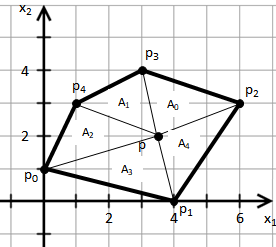
\includegraphics[]{simplex}
\end{figure}

$A_0 = \begin{vmatrix}
			6 & 3 &  3.5 \\
			3 & 4 &  2   \\
			1 & 1 &  1   \\
		\end{vmatrix} = 5.5 $
		\newline
		\newline
$A_1 = \begin{vmatrix}
			3 & 1 &  3.5 \\
			4 & 3 &  2   \\
			1 & 1 &  1   \\
		\end{vmatrix} = 4.5 $
		\newline
		\newline
$A_2 = \begin{vmatrix}
			1 & 0 &  3.5 \\
			3 & 1 &  2   \\
			1 & 1 &  1   \\
		\end{vmatrix} = 6 $
		\newline
		\newline
$A_3 = \begin{vmatrix}
			0 & 4 &  3.5 \\
			1 & 0 &  2   \\
			1 & 1 &  1   \\
		\end{vmatrix} = 7.5 $
		\newline
		\newline
$A_4 = \begin{vmatrix}
			4 & 6 &  3.5 \\
			0 & 3 &  2   \\
			1 & 1 &  1   \\
		\end{vmatrix} = 5.5 $
		\newline
		\newline
$A_{ges} = A_0 + A_1 + A_2 + A_3 + A_4$
\begin{align*}
\lambda_0 = \frac{A_0}{A_{ges}} = \frac{0.5 \cdot 5.5}{0.5 \cdot 29} & = 0.1900 \\
\lambda_1 = \frac{A_1}{A_{ges}} =\frac{0.5 \cdot 4.5}{0.5 \cdot 29} & = 0.1552 \\
\lambda_2 = \frac{A_2}{A_{ges}} =\frac{0.5 \cdot 6}{0.5 \cdot 29}   & = 0.2070 \\
\lambda_1 = \frac{A_3}{A_{ges}} =\frac{0.5 \cdot 7.5}{0.5 \cdot 29} & = 0.2586 \\
\lambda_4 = \frac{A_4}{A_{ges}} =\frac{0.5 \cdot 5.5}{0.5 \cdot 29} & = 0.1900 \\
\end{align*}
$$ p_{BAR} = \left( \frac{5.5}{29}, \frac{4.5}{29}, \frac{6}{29}, \frac{7.5}{29}, \frac{5.5}{29} \right)  ^T $$

\subsection{Tragen Sie in die folgende Zeichnung für alle gelb markierten Punkte die baryzentrischen Koordinaten bezogen auf die jeweiligen drei Punkte $A$, $B$ und $C \in \mathbb{R}^2$ ein.}

\begin{figure}[!htbp]
	\centering						
	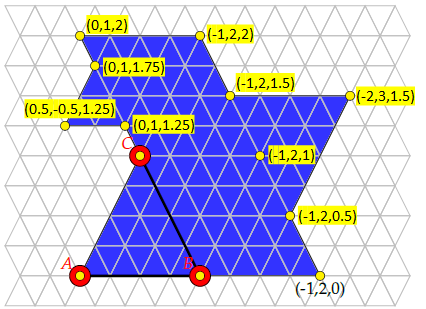
\includegraphics[width=0.95\linewidth]{map2}
\end{figure}


\section{Räumliche Datenstrukturen}

\subsection{Für Hüllenkörperhierarchien, Reguläre Gitter und Octrees seinen folgende naiven Ansätze vorgegeben, welche beschreiben, welche Anpassungen vorgenommen werden, sobald ein Objekt im Raum bewegt wird.}

\begin{itemize}
	\item Hüllenkörperhierarchien: Das Bounding Volume (BV) des Objekts selbst wird für die neue Position neu berechnet und ersetzt das alte BV in der Hierarchie. Die in der Hierarchie übergeorneten BVs werden entsprechend vergrößert bzw. verkleinert, sodass das neue BV des verschobenen Objekts vollständig enthalten ist.
	\item Reguläre Gitter: Das Objekt wird aus allen Zellen entfernt in denen es nicht mehr enthalten ist und wird zu allen Zellen hinzugefügt in denen es neu enthalten ist.
	\item Octree: Genauso wie bei Regulären Gittern
\end{itemize}

Erklären Sie für alle drei Datenstrukturen ob und warum diese Änderungen für dynamische Szenen ausreichend sind. Überlegen Sie sich insbesondere inwiefern der Zweck der Datenstruktur (die beschleunigte Suche von Objekten im Raum) weiter erfüllt wird.

\begin{itemize}
\item Hüllenkörperhierarchien: Die Schritte sind ausreichend, da durch anpassen der übergeordneten Volumen die Hierarchie korrekt bleibt. Das Culling kann also immer noch korrekt ausgeführt werden.
\item Reguläre Gitter:  Die Änderungen sind ausreichend, da eine Zelle als einzige Information enthält, welche Elemente enthalten sind. Der Zweck der beschleunigten Suche wird weiter erfüllt, da der Zugriff auf Nachbar-Zellen sehr schnell und damit auch das Update schnell durchgeführt werden kann.
\item Octree: Die Zellen beim Octree sind an die gegebenen Objekte im Raum angepasst. Demnach reicht der beschriebene Ansatz zwar aus, liefert aber unter Umständen weniger schnell ein Ergebnis in dynamischen Szenen.
\end{itemize}

\subsection{Gegeben ist eine 2D-Szene mit Objekten, wobei jedes Symbol ein Objekt repräsentiert. Weiterhin gegeben ist eine KD-Tree-Zerlegung dieser Szene. Die Buchstaben kennzeichnen die Geraden, die die Halbebenen voneinander abtrennen.}

\begin{figure}[!htbp]
	\centering
	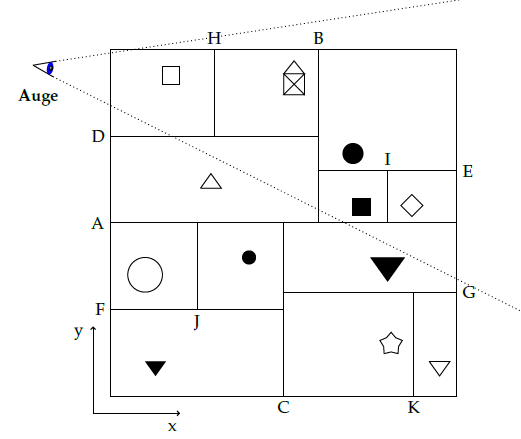
\includegraphics[]{scene}
\end{figure}

Zeichnen Sie den dazugehörigen Baum dieser Szene. Gehen Sie dabei so vor, dass der linke Teilbaum den Raum mit kleineren Koordinaten enthält, der rechte Teilbaum den Raum mit größeren Koordinaten. In den Blättern soll jeweils ein Objekt enthalten sein.

\begin{figure}[!htbp]
	\centering
	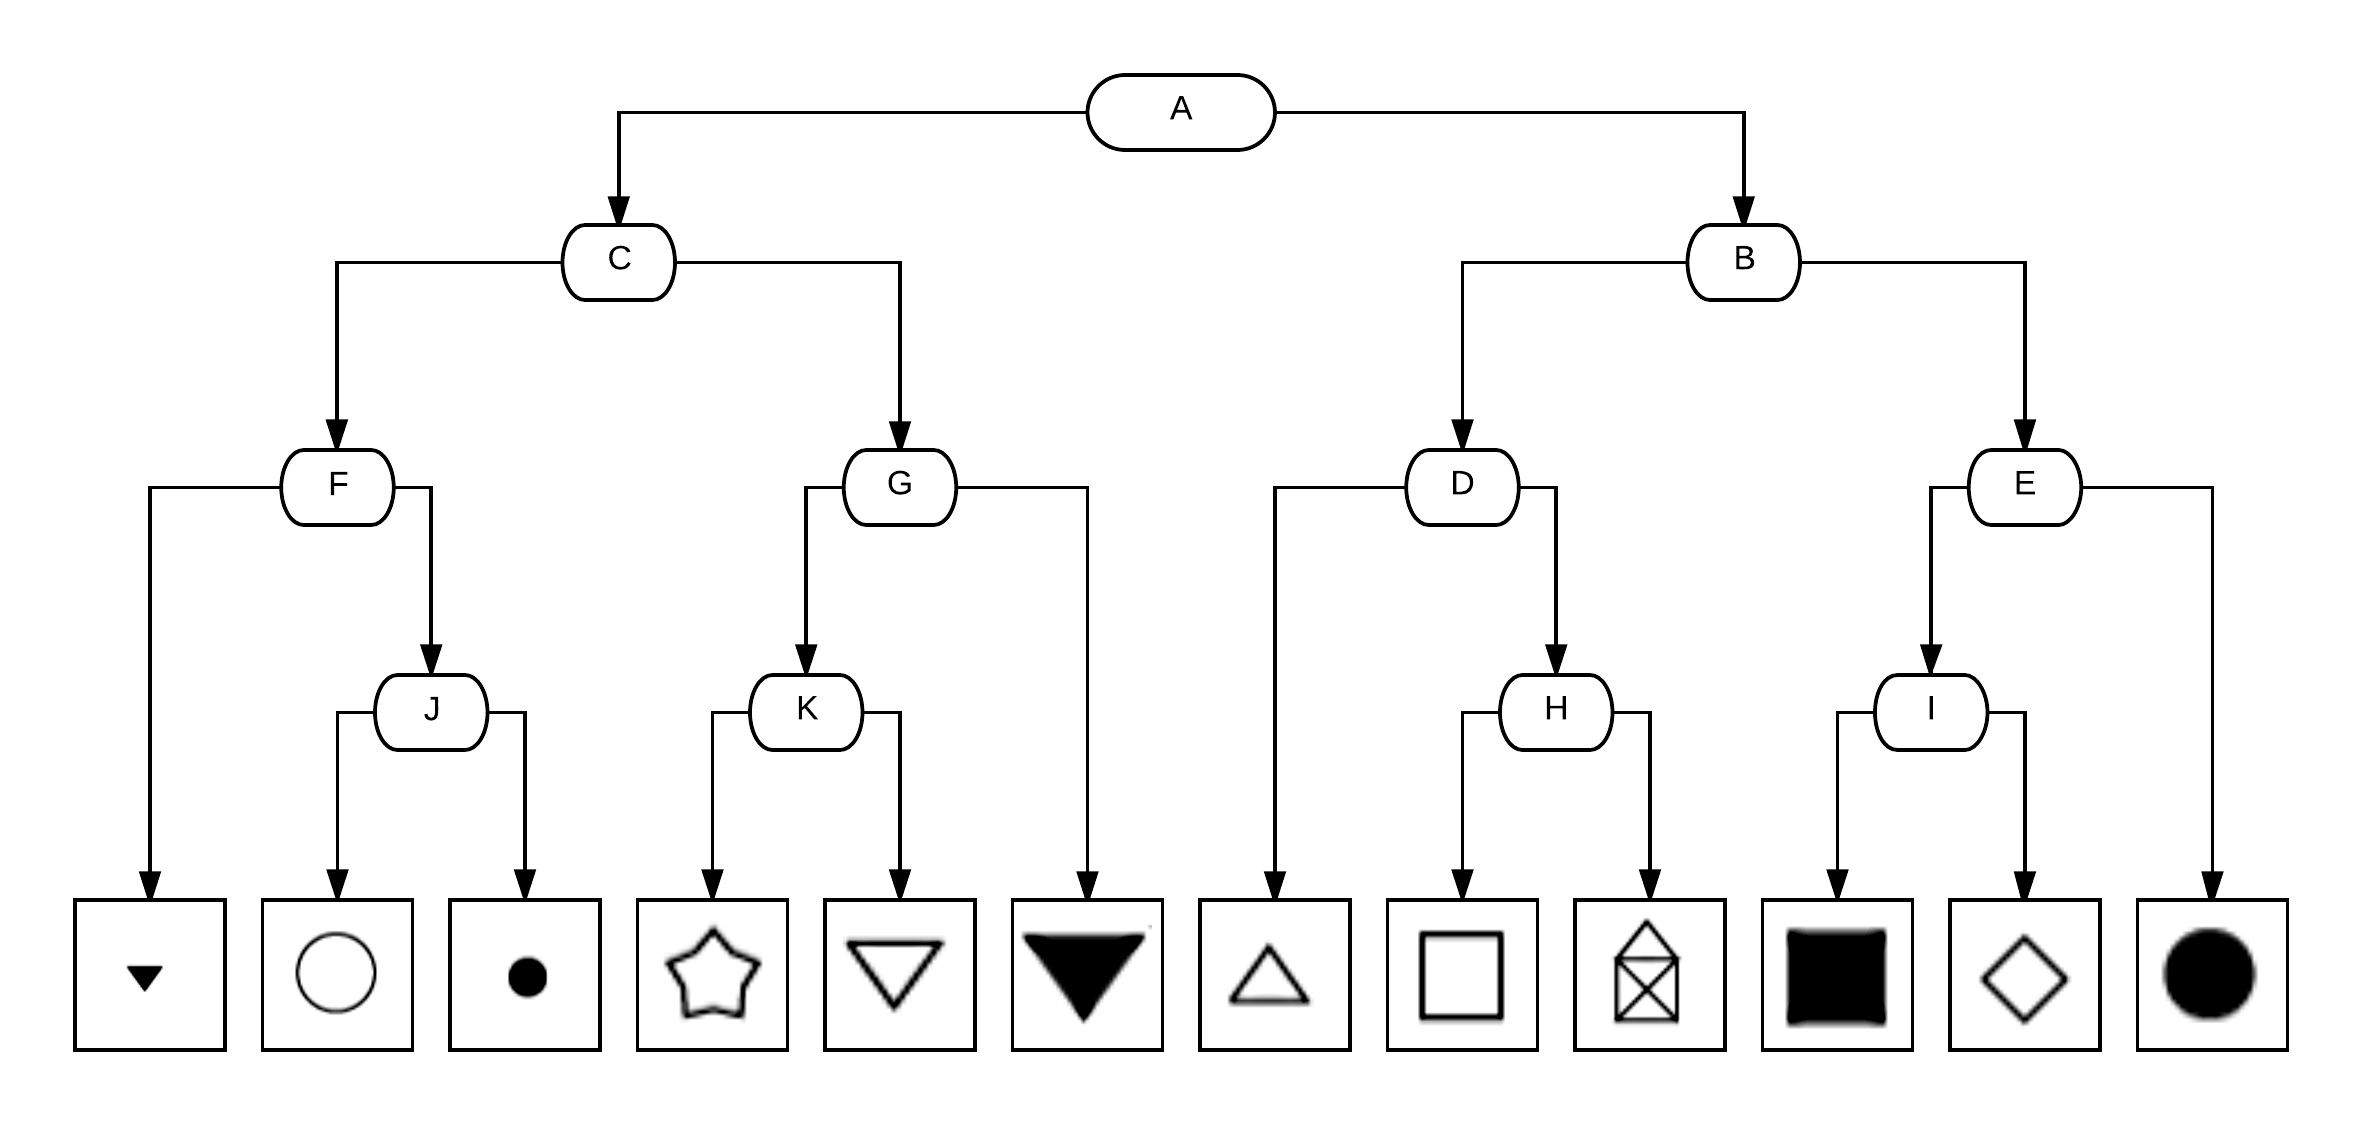
\includegraphics[width=1\linewidth]{kd}
\end{figure}

\newpage
\subsection{Welche Teilbäume des KD-Trees können für das in b) eingezeichnete View-Frustum verworfen werden?}

\begin{figure}[!htbp]
	\centering
	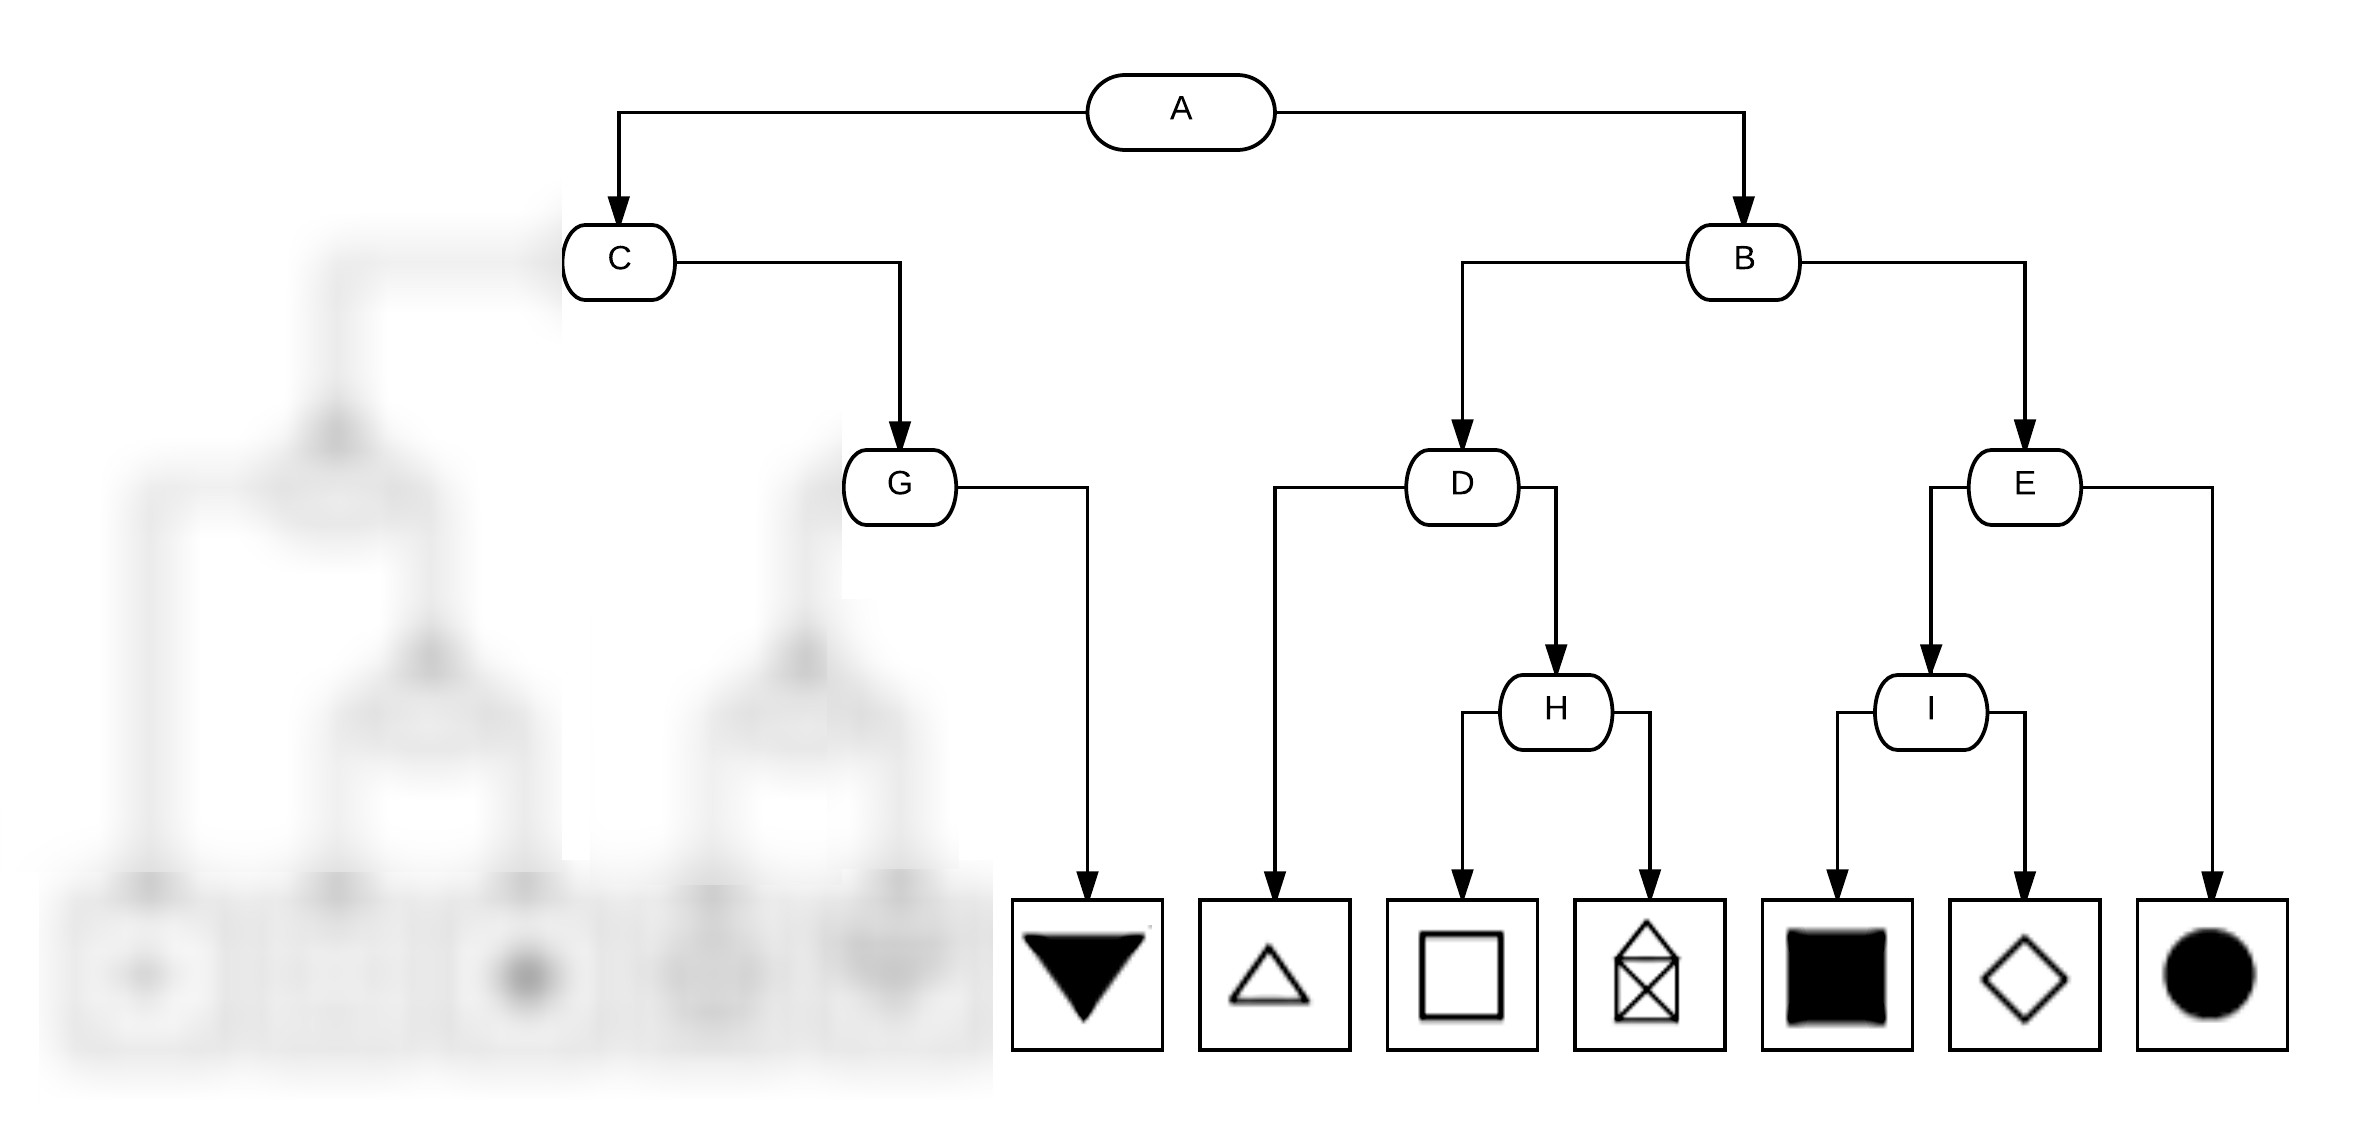
\includegraphics[width=1\linewidth]{kd_blur}
	\caption*{Die verschwommenen Teilbäume $F$, $J$ unud $K$ können verworfen werden.}
\end{figure}

\end{document}
